%
%picagelb
\subsection{Deutung eines Kurvenverlaufs}
	\begin{figure}[h]
		\begin{center}
		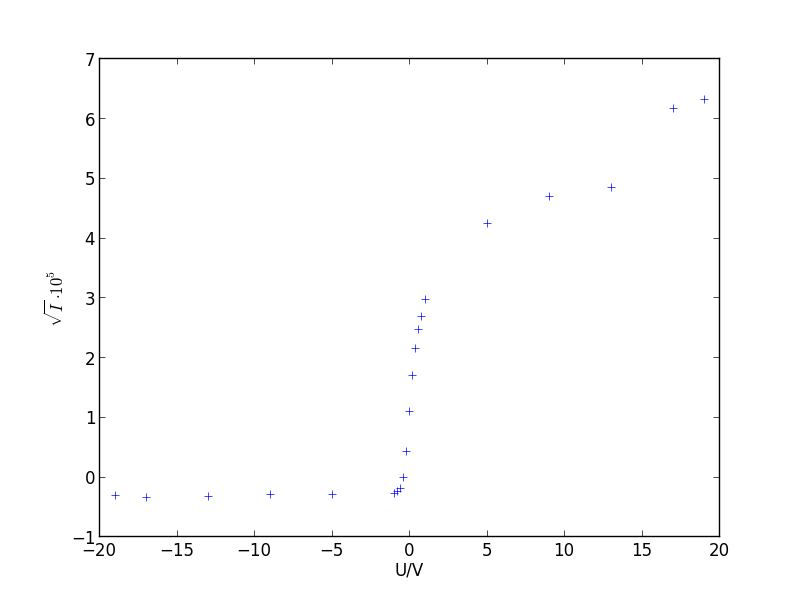
\includegraphics[scale=0.7]{picagelb.jpg}
		\caption{Photostrom in Abhängigkeit der angelegten Spannung ($\lambda=492$ nm)}
		\label{picagelb}
		\end{center}	
	\end{figure}
In Abbildung \ref{picagelb} ist für $\lambda=578\text{ nm}$ der Photostrom abhängig der
angelegten Spannung aufgetragen. Es ist bei hohen beschleunigenden Spannungen ein
Sättigungsverhalten zu erkennen, dem zu Grunde liegt die Eigenschaft, dass die Anzahl der
ausgelösten Elektronen von der Intesität des Lichtes abhängt. Das Ohmschen Gesetz lässt sich in diesem Fall 
nicht anwenden, da die Elektronen zur Anode hin beschleunigt werden. Dieser Sättigungswert hängt neben
der Intensität des Lichtes auch von der bestrahlten Fläche und den Materialeigenschaften ab. Dabei liegt 
die Asymptotik an dem Unvermögen der Versuchsanordnung alle Elektronen zu registrieren. Damit wirklich 
alle Elektronen die Anode erreichen, müsste der Abstand zwischen Anode und Kathode gegen Null
streben, was natürlich ein solches Experiment nicht möglich machen würde.\\ 
Der Photostrom nähert sich bereits bei $U>U_g$ an 0 V an, da die Elektronen nach der Fermi-Dirac 
Statistik verteilt sind und es so auch Elektronen gibt, die bei $U>U_g$ gar nicht erst genug
Energie besitzen die Anode zu erreichen. Der entgegengerichtete Photostrom von ungefähr -0,01 nA 
kommt durch den an der Anode stattfindenden Photoeffekt zustande. Da die bestrahlte Oberfläche der 
Anode wesentlich kleiner ist, wird schon bei relativ kleinen Spannungsbeträgen eine Sättigung erreicht.
Die Austrittsarbeit der Anode ist gering, denn schon bei Einstrahlung energiearmen Lichtes 
($\lambda \approx 650$ nm)\cite{anleitung} tritt bereits ein negativer Photostrom auf.

\subsection{Fehleranalyse und Literaturvergleich}
Das experimentell bestimmte Verhältnis von $h/e_0=(3,8\pm0,3)\cdot10^{-15}\text{ }\frac{\text{J$\cdot$s}}{\text{C}}$
passt zu dem Literaturwert \cite{tafel} von $h/e_0=4,1\cdot10^{-15}\text{ }\frac{\text{J$\cdot$s}}{\text{C}}$.
Ebenso passt der experimentell bestimmte Wert für die Austrittsarbeit von $A_k=(1,58\pm0,07)\text{ eV}$
grundsätzlich zu der erwarteten Größenordnung für die Austrittsarbeiten von Metallen.
Die auftretenden Abweichungen können viele Ursachen haben:
Zum einen war der Schwenkarm der Anordnung leicht versehentlich zu verschieben, zum anderen war die Versuchsanordnung unzureichend von
störenden Lichteinflüssen, wie Schreibleuchten, geschützt. Vor allem jedoch hatte das Messgerät des
Photostroms die Eigenschaft einen stark schwankenden Wert anzuzeigen. Das alles wirkt sich natürlich 
deutlich auf das Versuchsergebnis aus, wodurch Abweichungen zu erklären wären. 